\documentclass[12pt,a4paper]{article}

\usepackage[margin=1in]{geometry}
\usepackage{amsmath, amssymb, amsthm}
\usepackage{enumitem}
\usepackage{booktabs}
\usepackage{tikz}
\usetikzlibrary{arrows.meta, positioning}

\setlength{\parindent}{0pt}
\setlength{\parskip}{6pt}

\newtheoremstyle{notestyle}
  {8pt}
  {8pt}
  {\normalfont}
  {}
  {\bfseries}
  {.}
  {0.5em}
  {}

\theoremstyle{notestyle}
\newtheorem{example}{Example}

\newenvironment{answer}
{\par\textbf{Answer.}\ }
{\hfill$\square$\par}

\title{\textbf{Clarification: Random Walk Return Probability and Stirling's Formula}}
\author{MA4034: Time Series and Stochastic Processes}
\date{}

\begin{document}
\maketitle

\section{The Random Walk Setup}

Consider a one-dimensional random walk on the integers:
\[
S=\{\ldots,-2,-1,0,1,2,\ldots\}.
\]

From any state $i$:
\[
i\to i+1
\quad\text{with probability }p,
\]
and
\[
i\to i-1
\quad\text{with probability }q=1-p.
\]

\begin{center}
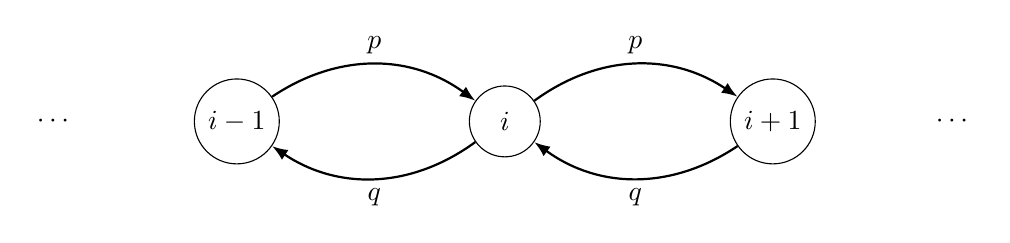
\begin{tikzpicture}[
  state/.style={circle, draw, minimum size=9mm},
  edge/.style={-{Latex[length=2mm]}, thick},
  bend angle=35
]
\node (leftdots) {$\cdots$};
\node[state, right=14mm of leftdots] (m1) {$i-1$};
\node[state, right=24mm of m1] (i) {$i$};
\node[state, right=24mm of i] (p1) {$i+1$};
\node[right=14mm of p1] (rightdots) {$\cdots$};

\draw[edge] (m1) edge[bend left] node[above] {$p$} (i);
\draw[edge] (i) edge[bend left] node[below] {$q$} (m1);
\draw[edge] (i) edge[bend left] node[above] {$p$} (p1);
\draw[edge] (p1) edge[bend left] node[below] {$q$} (i);
\end{tikzpicture}
\end{center}

We want to find:
\[
p_{ii}^{(2n)}
=
\Prob(X_{2n}=i\mid X_0=i).
\]

This means:
\[
\text{starting at }i,\text{ what is the probability of being back at }i\text{ after }2n\text{ steps?}
\]

\section{Why Must the Number of Steps Be Even?}

To return to the same state, the number of right steps must equal the number of left steps.

For example, if we start at $0$:
\[
R = \text{one step right},\qquad L=\text{one step left}.
\]

The path
\[
R,L
\]
returns to 0.

The path
\[
R,R,L,L
\]
also returns to 0.

But the path
\[
R,L,R
\]
does not return to 0, because there are two right steps and one left step.

So to return to the starting state, we need:
\[
\#R=\#L.
\]

Therefore, the total number of steps must be even:
\[
2n=n+n.
\]

\section{Why Do We Need $n$ Right Steps and $n$ Left Steps?}

Suppose the walk takes $2n$ steps and returns to the same state.

Let
\[
r=\text{number of right steps}
\]
and
\[
\ell=\text{number of left steps}.
\]

Since there are $2n$ total steps:
\[
r+\ell=2n.
\]

To return to the starting state, right steps and left steps must cancel:
\[
r=\ell.
\]

Solving these two equations:
\[
r+\ell=2n,
\qquad
r=\ell.
\]

Substitute $\ell=r$:
\[
r+r=2n.
\]
So
\[
2r=2n,
\]
and hence
\[
r=n.
\]
Therefore,
\[
\ell=n.
\]

So a return after $2n$ steps must contain:
\[
n\text{ right steps}
\]
and
\[
n\text{ left steps}.
\]

\section{Where Does $\binom{2n}{n}$ Come From?}

After $2n$ steps, we need exactly $n$ right steps and $n$ left steps.

The question is:

\[
\text{How many different orders can these steps appear in?}
\]

For example, if $2n=4$, then $n=2$. We need two $R$'s and two $L$'s.

The possible orders are:
\[
RRLL,\quad RLRL,\quad RLLR,\quad LLRR,\quad LRLR,\quad LRRL.
\]

There are 6 possible orders.

Using combinations:
\[
\binom{4}{2}=6.
\]

Why?

Because among 4 positions, we choose which 2 positions are right steps. The remaining 2 positions automatically become left steps.

For general $2n$ steps:
\[
\text{choose }n\text{ positions for the right steps out of }2n\text{ positions}.
\]

Therefore, the number of possible orders is
\[
\binom{2n}{n}.
\]

Using the factorial formula:
\[
\binom{2n}{n}=\frac{(2n)!}{n!n!}.
\]

\section{Why is Each Path Probability $p^nq^n$?}

Each right step has probability $p$.

Each left step has probability $q=1-p$.

For a returning path after $2n$ steps, there are:
\[
n\text{ right steps}
\]
and
\[
n\text{ left steps}.
\]

So the probability of one particular order is
\[
p^nq^n.
\]

For example:
\[
RRLL
\]
has probability
\[
p\cdot p\cdot q\cdot q=p^2q^2.
\]

Also:
\[
RLRL
\]
has probability
\[
p\cdot q\cdot p\cdot q=p^2q^2.
\]

Every valid returning path has the same probability:
\[
p^nq^n.
\]

\section{Final Formula for Return Probability}

There are
\[
\binom{2n}{n}
\]
valid returning paths.

Each has probability
\[
p^nq^n.
\]

Therefore,
\[
p_{ii}^{(2n)}
=
\binom{2n}{n}p^nq^n.
\]

Since
\[
q=1-p,
\]
we can write
\[
p_{ii}^{(2n)}
=
\binom{2n}{n}p^n(1-p)^n.
\]

Using factorials:
\[
p_{ii}^{(2n)}
=
\frac{(2n)!}{n!n!}\{p(1-p)\}^n.
\]

\section{Worked Small Examples}

\begin{example}
Find the probability of returning to the starting state after 2 steps.
\end{example}

\begin{answer}
Here,
\[
2n=2,
\]
so
\[
n=1.
\]

We need one right step and one left step.

The possible orders are:
\[
RL,\quad LR.
\]

There are
\[
\binom{2}{1}=2
\]
orders.

Each path has probability
\[
pq.
\]

Therefore,
\[
p_{ii}^{(2)}=2pq.
\]
\end{answer}

\begin{example}
Find the probability of returning to the starting state after 4 steps.
\end{example}

\begin{answer}
Here,
\[
2n=4,
\]
so
\[
n=2.
\]

We need two right steps and two left steps.

The number of possible orders is
\[
\binom{4}{2}=6.
\]

Each path has probability
\[
p^2q^2.
\]

Therefore,
\[
p_{ii}^{(4)}=6p^2q^2.
\]
\end{answer}

\begin{example}
If $p=0.4$, find the probability of returning to the starting state after 4 steps.
\end{example}

\begin{answer}
Here,
\[
p=0.4,\qquad q=0.6.
\]

From the previous example:
\[
p_{ii}^{(4)}=6p^2q^2.
\]

Substitute:
\[
p_{ii}^{(4)}
=
6(0.4)^2(0.6)^2.
\]

So
\[
p_{ii}^{(4)}
=
6(0.16)(0.36)
=
0.3456.
\]
\end{answer}

\section{Why Use Stirling's Formula?}

The exact formula is
\[
p_{ii}^{(2n)}
=
\frac{(2n)!}{n!n!}\{p(1-p)\}^n.
\]

This is exact, but it is hard to understand when $n$ is very large because factorials become huge.

Stirling's formula gives a simpler approximation:
\[
n!\sim n^ne^{-n}\sqrt{2\pi n}.
\]

This means:
\[
n!\text{ behaves approximately like }n^ne^{-n}\sqrt{2\pi n}
\]
when $n$ is large.

\section{Using Stirling's Formula Step by Step}

Start with
\[
\binom{2n}{n}
=
\frac{(2n)!}{n!n!}.
\]

Using Stirling's formula:
\[
(2n)!\sim (2n)^{2n}e^{-2n}\sqrt{2\pi(2n)}.
\]

So
\[
(2n)!\sim (2n)^{2n}e^{-2n}\sqrt{4\pi n}.
\]

Also,
\[
n!\sim n^ne^{-n}\sqrt{2\pi n}.
\]

Therefore,
\[
n!n!\sim
\left(n^ne^{-n}\sqrt{2\pi n}\right)^2.
\]

So
\[
n!n!\sim n^{2n}e^{-2n}(2\pi n).
\]

Thus,
\[
\binom{2n}{n}
\sim
\frac{(2n)^{2n}e^{-2n}\sqrt{4\pi n}}
{n^{2n}e^{-2n}(2\pi n)}.
\]

Cancel $e^{-2n}$:
\[
\binom{2n}{n}
\sim
\frac{(2n)^{2n}\sqrt{4\pi n}}
{n^{2n}(2\pi n)}.
\]

Now,
\[
\frac{(2n)^{2n}}{n^{2n}}=2^{2n}=4^n.
\]

Also,
\[
\sqrt{4\pi n}=2\sqrt{\pi n}.
\]

Therefore,
\[
\binom{2n}{n}
\sim
\frac{4^n\cdot 2\sqrt{\pi n}}{2\pi n}.
\]

Cancel 2:
\[
\binom{2n}{n}
\sim
\frac{4^n\sqrt{\pi n}}{\pi n}.
\]

Since
\[
\frac{\sqrt{\pi n}}{\pi n}=\frac1{\sqrt{\pi n}},
\]
we get
\[
\binom{2n}{n}
\sim
\frac{4^n}{\sqrt{\pi n}}.
\]

\section{Applying This to Return Probability}

Recall:
\[
p_{ii}^{(2n)}
=
\binom{2n}{n}p^n(1-p)^n.
\]

Using
\[
\binom{2n}{n}
\sim
\frac{4^n}{\sqrt{\pi n}},
\]
we get
\[
p_{ii}^{(2n)}
\sim
\frac{4^n}{\sqrt{\pi n}}p^n(1-p)^n.
\]

Combine the powers:
\[
4^np^n(1-p)^n
=
\{4p(1-p)\}^n.
\]

Therefore,
\[
\boxed{
p_{ii}^{(2n)}
\sim
\frac{\{4p(1-p)\}^n}{\sqrt{\pi n}}.
}
\]

\section{Why This Helps with Recurrence}

To check recurrence, we study
\[
\sum_{n=1}^{\infty}p_{ii}^{(n)}.
\]

For a random walk, odd return probabilities are zero:
\[
p_{ii}^{(2n-1)}=0.
\]

So we only care about
\[
\sum_{n=1}^{\infty}p_{ii}^{(2n)}.
\]

Using the approximation:
\[
p_{ii}^{(2n)}
\sim
\frac{\{4p(1-p)\}^n}{\sqrt{\pi n}}.
\]

\subsection*{Case 1: $p=\frac12$}

If
\[
p=\frac12,
\]
then
\[
4p(1-p)
=
4\left(\frac12\right)\left(\frac12\right)
=1.
\]

So
\[
p_{ii}^{(2n)}
\sim
\frac1{\sqrt{\pi n}}.
\]

The series
\[
\sum_{n=1}^{\infty}\frac1{\sqrt{n}}
\]
diverges.

Therefore the fair one-dimensional random walk is recurrent.

But the expected return time is infinite, so it is null recurrent.

\subsection*{Case 2: $p\neq\frac12$}

If
\[
p\neq\frac12,
\]
then
\[
4p(1-p)<1.
\]

Let
\[
r=4p(1-p).
\]

Then
\[
0<r<1.
\]

So
\[
p_{ii}^{(2n)}
\sim
\frac{r^n}{\sqrt{\pi n}}.
\]

Because $r^n$ decreases geometrically, the series converges.

Therefore the biased one-dimensional random walk is transient.

\section{Practice Questions}

\begin{enumerate}[label=\textbf{Q\arabic*.}, leftmargin=1.2cm]
    \item Starting from state $0$, list all paths that return to $0$ after 2 steps.

    \item Starting from state $0$, how many paths return to $0$ after 6 steps?

    \item Write the formula for the probability of returning to the starting state after 6 steps.

    \item If $p=0.5$, find $p_{ii}^{(4)}$.

    \item If $p=0.3$, find $p_{ii}^{(2)}$.

    \item Explain why $\binom{2n}{n}$ appears in the return probability formula.

    \item Use Stirling's approximation to state what $\binom{2n}{n}$ behaves like for large $n$.

    \item If $p=0.5$, what does
    \[
    p_{ii}^{(2n)}
    \]
    behave like for large $n$?

    \item If $p=0.4$, is the one-dimensional random walk recurrent or transient? Explain using $4p(1-p)$.
\end{enumerate}

\section{Answers}

\subsection*{Answer 1}

To return to 0 after 2 steps, we need one right step and one left step.

The possible paths are:
\[
RL,\quad LR.
\]

\subsection*{Answer 2}

Returning after 6 steps means
\[
2n=6.
\]
So
\[
n=3.
\]

We need 3 right steps and 3 left steps.

The number of possible paths is
\[
\binom{6}{3}=20.
\]

\subsection*{Answer 3}

After 6 steps, we need 3 right steps and 3 left steps.

Thus,
\[
p_{ii}^{(6)}
=
\binom{6}{3}p^3q^3.
\]

Since
\[
\binom{6}{3}=20,
\]
we get
\[
p_{ii}^{(6)}=20p^3q^3.
\]

\subsection*{Answer 4}

For 4 steps,
\[
p_{ii}^{(4)}=\binom{4}{2}p^2q^2.
\]

If
\[
p=0.5,
\]
then
\[
q=0.5.
\]

Therefore,
\[
p_{ii}^{(4)}
=
6(0.5)^2(0.5)^2
=
6\left(\frac14\right)\left(\frac14\right)
=
\frac{6}{16}
=
\frac38.
\]

\subsection*{Answer 5}

For 2 steps,
\[
p_{ii}^{(2)}=2pq.
\]

If
\[
p=0.3,
\]
then
\[
q=0.7.
\]

So
\[
p_{ii}^{(2)}
=
2(0.3)(0.7)
=
0.42.
\]

\subsection*{Answer 6}

To return after $2n$ steps, we need exactly $n$ right steps and $n$ left steps.

There are $2n$ positions in the path. We choose which $n$ of those positions are right steps. The remaining $n$ positions are left steps.

Therefore the number of possible orders is
\[
\binom{2n}{n}.
\]

\subsection*{Answer 7}

Using Stirling's formula,
\[
\binom{2n}{n}
\sim
\frac{4^n}{\sqrt{\pi n}}.
\]

\subsection*{Answer 8}

If
\[
p=0.5,
\]
then
\[
4p(1-p)=1.
\]

Therefore,
\[
p_{ii}^{(2n)}
\sim
\frac1{\sqrt{\pi n}}.
\]

\subsection*{Answer 9}

If
\[
p=0.4,
\]
then
\[
4p(1-p)=4(0.4)(0.6)=0.96.
\]

Since
\[
0.96<1,
\]
the return probabilities behave like
\[
\frac{0.96^n}{\sqrt{\pi n}}.
\]

This series converges because of the geometric factor $0.96^n$.

Therefore the random walk is transient.

\end{document}
